\section{Facial Detection and Recognition}
%% TODO: Brian dump ur stuff here

Since simple image operations mentioned earlier can be done within a homomorphic cryptosystem, these operations can be assembled together in order to do more complex operations. A prominent application of image processing that often uses complex image operations is \textit{facial recognition}.

Traditional facial recognition algorithms rely on detecting salient features in a face image. Two of the popular facial recognition algorithms are \textit{eigenfaces} and \textit{Haar cascades}.

\subsection{Eigenfaces}

Proposed by Matthew Turk and Alex Pentland, the eigenfaces method uses principal component analysis (PCA) in order to express an input image as a linear combination of eigenfaces \cite{turk_eigenfaces_1991}. An \textit{eigenface} is a principal component, or more simply an eigenvector that represents a certain variation between the face images which are taken from the initial training set. The number of resulting eigenfaces is equal to the number of face images in the training set.

In the enrollment process, $M$ face images $\Theta_1, \ldots, \Theta_M$, each of size $p \times q$, are taken in to comprise the initial training set. The training images can be represented as vectors of length $N = pq$, where each row of an image is concatenated together.

The average of the training images, denoted as $\Psi$, is 
\[ \Psi = \frac{1}{M} \sum_{i=1}^{M} \Theta_i \]

The \textit{difference vectors} are then computed as $\Phi_i = \Theta_i - \Psi$. PCA is applied on the covariance matrix of the vectors
\[ \mathbf{C} = \frac{1}{M} \sum_{i=1}^M \Phi_i \Phi_i^\top = \frac{1}{M} \mathbf{A}\mathbf{A}^\top,\]
where $\mathbf{A}$ is an $N \times M$ matrix defined by $\left[\Theta_1 \quad \Theta_2 \quad \cdots \quad \Theta_M\right]$, in order to determine the orthonormal eigenvectors \cite{hutchison_privacy-preserving_2009}.

Directly computing the covariance matrix and then applying PCA will become inefficient for large sizes of $\mathbf{A}$, since computing for $\mathbf{A}\mathbf{A}^\top$ results in an $N \times N$ matrix, which can get drastically large because it is dependent on the size of the image. On the other hand, computing for $\mathbf{A}^\top\mathbf{A}$ only results in an $M \times M$ matrix, which is much smaller than the previous one because it is just dependent on the number of face images in the training set. Now, we can apply PCA to $\mathbf{A}^\top\mathbf{A}$ along with some post-processing to obtain the eigenvectors \cite{hutchison_privacy-preserving_2009}. 

Instead of getting the eigendecomposition of the covariance matrix by explicitly computing the eigenvalues and eigenvectors of $\mathbf{C}$, we can also apply \textit{singular value decomposition} (SVD) on the matrix $\Phi^\top$. This is because SVD works through a divide-and-conquer method which results in greater numerical stability, while eigendecomposition simply uses the traditional QR factorization \cite{nakatsukasa_stable_2013, gu_divide-and-conquer_1995}. Upon applying SVD, we now get the eigenvectors $\mathbf{u}_1, \ldots, \mathbf{u}_M$ and their corresponding eigenvalues $\lambda_1, \ldots, \lambda_M$.

We choose $K$ eigenvectors $\mathbf{u}_1, \ldots, \mathbf{u}_K$ such that it comprises a set associated with the $K$ largest eigenvalues, where $K$ is much smaller than $M$. This set is now the \textit{face space}. Then, the images $\Theta_1, \ldots, \Theta_K$ are projected onto the face space spanned by the eigenfaces to determine the weight vectors $\Omega_1, \ldots, \Omega_K$.

To perform the recognition process, the algorithm projects the input image $\Gamma$ onto the face space, and then comparing the projected image $\bar{\Omega} = \mathbf{u}_i\left(\Gamma - \Psi\right)$ with each eigenface in the face space using a metric such as the Euclidean distance. Thus it is computed as $d_i = \left\lVert \Omega_i -\bar{\Omega} \right\rVert$ for all $i=1,\ldots,K$, where $\left\lVert \cdot \right\rVert$ denotes the Euclidean norm.

Then, a match can be reported if the smallest possible distance is smaller than the given threshold value $T$. 
\newcommand{\argmin}{\mathop{\mathrm{arg\,min}}}  
\[\text{ID} = \begin{cases}\argmin_i d_i & \text{if } \min_i d_i \le T \\\emptyset & \text {otherwise}\end{cases}
\]

\subsection{Haar Cascades}
A \textit{Haar cascade classifier} is another method for facial recognition by Paul Viola and Michael Jones \cite{viola_robust_2004}. It uses Haar-like features to detect regularities in a face image. A \textit{Haar-like feature} looks at a certain rectangular region of the image through a filter-like window.

\begin{figure}[!h]
    \centering
    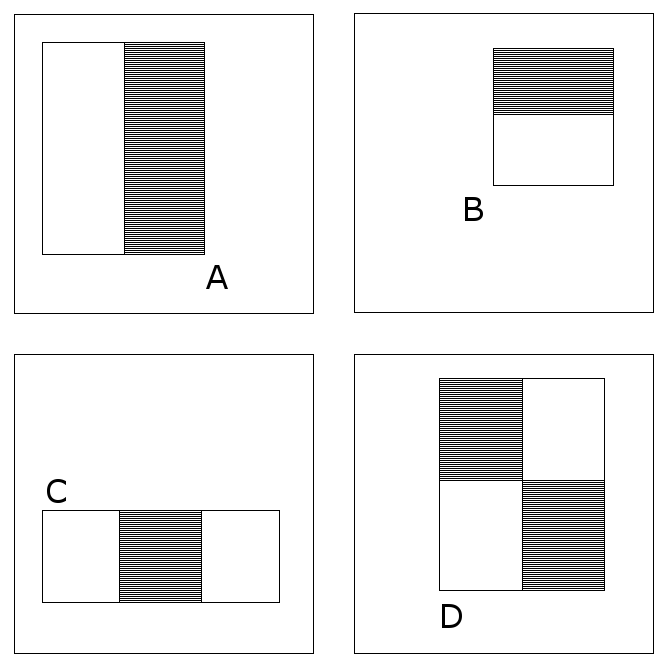
\includegraphics[width=7cm]{figures/haarfeatures2.png}
    \caption{Examples of Haar-like features \cite{viola_robust_2004}.}
\end{figure}

A Haar-like feature is composed of black and white rectangles, and arranged such that it detects a presence or an absence of a particular image feature or regularity of interest. For example, a feature may detect the difference in intensities between the eyes and the cheeks, another feature would detect the edges of the face, and another one would detect depending on the location of the eyes. The detection is done by summing up the intensities within the black region and the white region, and then calculating the difference.

Getting the sum of pixel intensities within a region na\"{i}vely would become inefficient as the size of the rectangular region increases, so a data structure called an \textit{integral image} is used to allow more efficient detection of Haar-like features. In other words, an integral image is essentially a two-dimensional range sum that can compute sums of rectangular regions in constant time, regardless of the size of the regions.

Most of the Haar-like features are irrelevant, because a feature that works in a certain part of the image would not necessarily work in another part. The whole process may become needlessly inefficient due to computational time being potentially wasted on a huge number of irrelevant features, even though computing for a feature is said to be efficient. That is why we need to select the best features and use those to form a strong classifier in a process called AdaBoost \cite{viola_robust_2004}.

In itself, a Haar-like feature is considered as a \textit{weak classifier}, the probability of detecting a certain feature is slightly greater than detecting at random \cite{viola_robust_2004}. So a large number of Haar-like features must be used together by forming them into cascade classifiers in order to achieve a sufficient enough accuracy. The resulting strong classifier would then be a linear combination of the weak classifiers.

Each stage in the cascade classifier consists of weak classifiers that uses decision stumps, so that the weak classifiers can classify many examples correctly. A \textit{decision stump} can be defined as
\[h \left(x, f, p, \theta \right) = \begin{cases}1 & \text{if } pf(x) < p\theta\\ 0 & \text{otherwise}\end{cases}
\]
where $x$ is a fixed window of the image, $f$ is the feature, $p$ is the polarity, and $\theta$ is the threshold \cite{viola_robust_2004}.

Each stage also labels the region as positive (meaning that there is a face within the region), and negative (if none). If the detector sees the region as negative, it is immediately discarded and not processed anymore. Otherwise if the region is labeled as positive, it moves to the next stage for further processing. When a region successfully completes all the stages, it can be considered as a face region.
